\documentclass[a4paper,10pt, english]{article}

\usepackage{amssymb}
\usepackage{amsmath}
\usepackage{enumitem}
\usepackage{graphicx}
\usepackage{subfig}
\usepackage{amsthm}




\newcommand{\D}{\displaystyle}

\newtheorem{theo}{Theorem}[section]
\newtheorem{dfn}{Definition}[section]
\newcommand{\R}{\mathbb{R}}
\newtheorem{prop}[theo]{Proposition}



















\begin{document}


\title{Decentrilized control for Cucker Smale system}
\author{}
\maketitle












\section{Introduction}
The aim of this work is to design a decentralized optimal control strategy for the Cucker-Smale system to steer the system to consensus while maintaining the spatial connectivity of the initial interaction graph.

Consider the Cucker-Smale system
\begin{align}
\begin{cases}
\D
\dot{x_i} = v_i,\\
\dot{v_i} = \frac{1}{N}\sum_{j\in \mathcal{I}}a(\|x_i - x_j\|)(v_j - v_i) + u_i, \\
x(0) = x_0,
v(0) = v_0.
\end{cases}
\label{csm}
\end{align}
where $i\in \mathcal{I} \subset \mathbb{N}$ \--- some set of indexes, $N = \# \mathcal{I}$ is the number of  $d$-dimensional agents, a pair $(x_i, v_i)\in \mathbb{R}^{2d}$, represents the position and velocity of every agent, $u_i$ is an external controller. This kind of model has been introduced by Cucker and Smale in [cucker-smale] for specific choices of the interaction function $a$ as
\begin{equation}
a(r) = \frac{1}{(1 + r^2)^\delta} \qquad \mbox{for every}\quad \delta \in [0, +\infty],
\label{a}
\end{equation}
this function defines the natural interaction force between agents. The unconditional consensus emergence largely depends on the strength of the force. In [cucker-smale] a result was presented related to the parameter $\delta$ in (\ref{a}); it asserts that for $\delta \leq 1/2$, the system tends asymptotically to consensus, independent of its initial configuration. For $\delta \geq 1/2$, consensus emergence will depend on the cohesion of the initial setting. A precise characterization of this situation was obtained in [9 from BFK] where a sufficient condition depending on the initial configuration and the parameter $\delta$ is provided. To state this condition let us define a symmetric bilinear form $B$ on $R^{N\times d} \times  R^{N\times d}$ by
\begin{equation}
B(u, v) = \frac{1}{2N^2}\sum_{i, j \in \mathcal{I}} \langle u_i - u_j, v_i - v_j  \rangle,
\label{b}
\end{equation}
where $\langle . \rangle$ denotes a scalar product in $R^d$.
\begin{theo}
Let $(x_0, v_0) \in R^{N\times d} \times  R^{N\times d}$ be such that $X_0 = B(x_0, x_0)$ and $V_0 = B(v_0, v_0)$ satisfy
$$
E(x_0, v_0):=\sqrt{V_0} - \int_{\sqrt{X_0}}^{\infty} a(\sqrt{2N}r)dr \leq 0.
$$
Then the solution of uncontrolled system (\ref{csm}) with initial data $(x_0, v_0)$  tends to consensus.
\end{theo}

There have been developed many analytical feedback control strategies  to steer the system (\ref{csm}) to consensus. In particular in [CFTP] it is shown that with a controller 
of the form
$$
u_i = \bar{v} - v_i,
$$
consensus emergence can be guaranteed for any configuration and values of $\delta$. A natural drawback of such a controller relates to the fact that is is always active, and it involves the whole system at every
instant of time. Later on,  in [BFK] a decentralized control setting  was studied \--- a local feedback depending on a metrical neighbourhood of the agents. The neighbours consist of all agents 
the distance to which is less than a specified number $R>0$
$$
u_i = \bar{v}_i - v_i,
$$
where $\bar{v}_i$ is an approximated mean velocity vector in the neighbourhood of radius $R$ instead of the true mean velocity of the whole group $\bar{v}$. This control guarantees the consensus emergence under certain initial conditions.




Let us define a distance dependent dynamic graph for the interactions between agents.
\begin{dfn}
We call $\mathcal{G}(t) =  (\mathcal{V}, \mathcal{E}(t) )$ a dynamic graph consisting of a set of vertices $\mathcal{V} = \{1, \dots,  N\}$ indexed by the set of agents and a time varying set of links 
$\mathcal{E}(t) = \{(i, j)|i, j \in \mathcal{V}\}$ such that, for any $R>0$
$$
\mbox{if}\quad 0<\|x_i(t) - x_j(t)\| \leq R \quad\mbox{then},\quad (i, j)\in \mathcal{E}(t).
$$
\end{dfn}
And let us denote $\mathcal{N}_i(t) = \{j|(i, j)\in\mathcal{E}(t)\}$ the neighbourhood of agent i.
Let us also denote an agent along with its neighbours as a set $\bar{\mathcal{N}}_i(t) = \mathcal{N}_i(t)\bigcup \{i\}$.
In [jadbabaieflocking while preserving connectivity] a distributed control law, based on potential fields, that achieve velocity alignment and maintain the existing links in the network was developed 
\begin{equation}
u_i = \bar{v}_i - v_i - \sum_{j \in \mathcal{N}_i(t)}\nabla_{x_i}V(\|x_i - x_j\|).
\label{controljad}
\end{equation}
where $\bar{v}_i = \sum_{j \in \mathcal{N}_i(t)} v_j$, and $V$ is an artificial potential function  to maintain the connectivity of the initial interaction graph $\mathcal{G}(0)$ 
\begin{equation}
 V(r) = \frac{1}{r^2} + \frac{1}{R^2 - r^2}, \qquad 0 < r < R.
\label{potential}
\end{equation}
This potential not only allows for maintaining links in the network but also for avoiding collisions among the agents. 

The drawback of the control (\ref{controljad}) is that it has an essential discontinuity as $r \longrightarrow R$ which on one hand guarantees network connection maintenance but on the other hand, as forces to break the network connectivity become stronger it requires increasingly fine mesh to be solved numerically, which renders it impractical for applications. We would like to design a decentralized control strategy with the same aims as (\ref{controljad}) but such that it avoids the continuity problem and is optimal in some sense. 
For this we consider minimizing the following objective functional 
\begin{equation}
J(x, v) = B(v(T), v(T)) + \int_{0}^{T}\sum_{(p, j)\in \mathcal{E}(t)} \bar{V}(\|x_p(t) - x_j(t)\|),
\label{Vt}
\end{equation}
where $B(v(T), v(T))$ stands for the consensus emergence at the terminal observation, and $\bar{V}$ is a potential that measures the relative distance between agents, which we would like to minimize
\begin{equation}
\bar{V}(r) = (R/N- r)^2, \qquad 0 < r.
\label{potentialbar}
\end{equation}
The idea of this potential is to increase the force with which the agents are pulled together as number of the agents increases, which would provide the increased connectivity of the network at the terminal configuration. Note, that we can not use the same potential as in (\ref{potential}) because the functional $J$ will not be coercive.



The decentralization strategy consists in decomposing the state domain in sub-domains $\bar{\mathcal{N}}_p(t)$ for every $p\in \mathcal{I}$ where an optimal control problem is solved independently to obtain the suitable decentralized control for agent $p$. Such decentralization has already been utilized for first order systems in [jadbabai decentralized control of connectivity].
The algorithm adopts the model predictive control approach by partitioning the time interval $[0, T]$ into $m$ time windows where subsequently solving an optimal control problem for each agent $p$.







 \subsection{The decentralized MPC strategy}
 
 The general idea of model predictive control is that future control inputs and future state are predicted using the system model and optimized at regular intervals. For
 the time interval $[0, T]$ where the evolution of system (\ref{csm}) is considered. 
 The time interval is partitioned into $m\in \mathbb{N}$ uniform time windows $[T_{l-1}, T_{l}]$, $l = 1, \dots, m$, $T_0 = 0, \dots, T_m = T$  of length  $\Delta T = T/m$. The genereal MPC strategy starts at zero time and solves the open-loop control problem defined in the interval $[T_0, T_1]$. Then, with response  resulting at time $T_1$ we have the initial condition for the subsequent optimization problem defined in the interval $[T_1, T_2]$. This procedure is repeated by receding the time horizon until the last window is reached. We implement the MPC scheme where the time horizon used to evaluate the control coincides with the time horizon where the control is used.
 
 The decentralization comes with state domain decomposition on each time window $[T_{l-1}, T_{l}]$, $l = 1, \dots, m$  of the MPC scheme where for each agent $p$, $p = 1, \dots, N$ we solve an optimal control problem for a state domain $\bar{\mathcal{N}}_p(T_{l-1})$ of the following form
  \begin{equation}
  \min_{x, v} J_p(x, v) = B(v(T_l), v(T_l)) + \int_{T_{l-1}}^{T_l}\sum_{j\in \mathcal{N}_p(T_{l-1})} \bar{V}(\|x_p(t) - x_j(t)\|),
 \label{opci}
 \end{equation}
 subject to (\ref{csm}) where $\mathcal{I} = \bar{\mathcal{N}}_p(T_l)$,  $N = N_p:= \# \bar{\mathcal{N}}_p(T_l)$, with initial conditions $(x(T_{l-1}), v(T_{l-1}))$ taken as endpoints form the solution on the previous time window $l-1$.
 Therefore, at each time window $l$ for each agent $p$ we obtain a suitable decentralized control $u_p(\mathcal{N}_p(T_l))$ which only depends on its neighbours in the time window $l$.
We assume the neighbourhood of agent $p$ does not change during evolution in time window $l$.

   The algorithm reads as the following: given the system (\ref{csm}):
   \begin{enumerate}
   \item Partition time interval $[0, T]$ into time windows $\Delta T$: $0 = T_0, T_1, \dots, T_m = T$.
   \item For each time window  $[T_{l-1}, T_{l}]$, $l = 1, \dots, m$ and for each agent $p$, $p = 1, \dots, N$  solve the OPC (\ref{opci}) with constrains (\ref{csm}) for the initial conditions $(x(T_{l-1}), v(T_{l-1}))$.
   \item From the solution of (\ref{opci}), (\ref{csm})  retrieve the  state for the agent $p$ in the time window $l$ $(x_p(t), v_p(t))$ and control $u_p(t)$, $t\in [T_{l-1}, T_{l}]$.
   \item Repeat the steps 2-3 until the solutions for all windows are obtained. 
 \end{enumerate}
 



 
 
 \section{The optimal contro problem and its discretization}
  We represent the optimal control problem  (\ref{opci}), (\ref{csm}) for agent $p$ on time window $[T_{l-1}, T_{l}]$ in Mayer form.
  
 \begin{align}
 \D
 & \mbox{minimize}\quad  C(X(T)),   \label{compact_cost} \\ 
 & \mbox{subject to} \quad \dot{X} = F(X(t), u(t)), \quad X(0) = X_0, \label{compact_equation}
 \end{align}
where  the control $u \in  L^{\infty}([T_{l-1}, T_{l}], \mathbb{R}^{N_p \times d})$,
the state $X\in H^1([T_{l-1}, T_{l}], \mathbb{R}^{N_p \times d} \times \mathbb{R}^{N_p\times d} \times \mathbb{R})$
in a compact form composed of the position and velocity 
states of (\ref{csm})   $X(t) = (x(t), v(t), z(t))$, $x(t) = (x_{i_1}(t), \dots, x_{i_{N_p}}(t))$,
 $v(t) = (v_{i_1}(t), \dots, v_{i_{N_p}}(t))$, $\{i_1, \dots, i_{N_p}\} \in \bar{\mathcal{N}}_p(T_l)$, 
 and $z(t)$ is an auxiliary component 
 $$
 z(t) =  \sum_{j\in \mathcal{N}_p(T_{l-1})} \bar{V}(\|x_p(t) - x_j(t)\|),
 $$
 with the initial condition $z(0) = 0$ and $F(X)$ is the dynamics of the system (\ref{csm}) in compact form
 $$
 F(X(t), u(t)) =
  \left( 
  \begin{array}{c}
  v(t)\\
   - L_xv(t) + u(t)\\
   z(t)\\
 \end{array} 
 \right), 
 $$
 where $L_x$ is the Laplacian of the $N_p\times N_p$ matrix $(a(\|x_i - x_j\|)/N_p)_{i, j\in\bar{\mathcal{N}}_p(T_{l-1})}$ which depends on $x$.
 For the functional $C$ to correspond to the problem in its original form it is chosen 
 $$
 C(X(T_l)) = z(T_l) + B(v(T_l), v(T_l)).
 $$
 
  Note, since our problem is autonomous and all time windows are of the same width, without loss of generality
 we can transform the problem on time interval $[0, \Delta T]$. 
 
 
  
  Given the problem (\ref{compact_cost} - \ref{compact_equation}) we discretize it with a third-order Runge-Kutta scheme.  For such scheme, the discrete controls often converge to the continuous solution slower than the discrete state and adjoint variables at the grid points. It  must satisfy an additional condition to achieve third-order accuracy
    for optimal control problems. Here, we utilise a better approximation to the continuous optimal control obtained from a posteriori computation involving the computed discrete state and adjoint variables  developed in [hager]. 
    
  Consider a uniform time mesh and the following time-step size
 \begin{equation}
   h = \frac{\Delta T}{n},
   \label{h}
 \end{equation}
 where $n$ is the total number of discrete time intervals in $[0, \Delta T]$.  The value of $X(t)$ at the discrete time $t_k$ is denoted with
 $$
 X^k = X(t^k), \qquad t^k = kh \quad\mbox{for} \quad k = 1, \dots n.
 $$
 For an $s$-stage Runge-Kutta discretization scheme it is defined by setting the coefficients $a_{ij}$ and
 $b_{i}$, $1\leq i, j\leq s$, such that they satisfy conditions given in [hager]. 
 
 Corresponding to the discretization setting, the optimal control problem (\ref{compact_cost} -  \ref{compact_equation})  attains the following form
 
 \begin{align}
  \D
  & \mbox{minimize}\quad C(X_n), \label{discrete_cost}\\
  & \mbox{subject to} \quad X^{k+1}  = X^k + h\sum_{i=1}^{s}b_iF(y^{ki}, u^{ki}), \qquad X_0 = X(0), \label{discrete_equation_x}\\
  & y^{ki} = X^k + h\sum_{j=1}^{s}a_{ij}F(y^{kj}, u^{kj}),\label{discrete_equation_y}
  \end{align}
 
 for $1\leq i, j\leq s$, and $0\leq k\leq n-1$.
 Where the vectors $y^kj$ and $u^{kj}$ are intermediate state and control variables on the interval $[t^k, t^{k+1}]$. The state uniqueness is guaranteed in [hager]. 
 
 
 

\newpage
\subsection{The gradient evaluation}
Provided the discrete OPC (\ref{discrete_cost} - \ref{discrete_equation_y}) the corresponding  optimality system  is given by

  \begin{align}
   \D
    & X^{k+1}  = X^k + h\sum_{i=1}^{s}b_iF(y^{ki}, u^{ki}), \qquad X_0 = X(0),   \label{os_state_x}\\
 	& y^{ki} = X^k + h\sum_{j=1}^{s}a_{ij}F(y^{kj}, u^{kj}),   \label{os_state_y}\\
 	& p^k = p^{k+1} + \sum_{i=1}^{s}\psi^{ki}, \qquad p^n = - \nabla_xC(X^n),  \label{os_adjoint_p}\\
 	& \psi^{ki} = (\nabla_x F(y^{ki}, u^{ki}))^{T} \left( p^{k+1} + \sum_{j=1}^{s} \frac{a_{ji}}{b_i}\psi^{kj}\right), \label{os_adjoint_psi} 
   \end{align}

The first order discrete system (\ref{os_state_x} - \ref{os_adjoint_psi}) provides a convenient way to compute the exact gradient of the discrete cost functional (\ref{discrete_cost})
\begin{equation}
\nabla_{u^{ki}} C(u) = - (\nabla_u F(y^{ki}, u^{ki}))^{T} \left( p^{k+1} + \sum_{j=1}^{s}\frac{a_{ji}}{b_i}\psi^{kj}\right), 
\label{discretegradient}
 \end{equation}  
 for $1\leq i, j\leq s$, and $0\leq k\leq n-1$, where the intermediate values for the discrete state and adjoint variables are obtained by first
 solving the discrete state equations (\ref{os_state_x} - \ref{os_state_y}) for $k=0, 1, \dots, n-1$, using the given values for the controls, and then using these computed values for both the state and intermediate variables in (\ref{os_adjoint_p} - \ref{os_adjoint_psi}) when computing the values of the discrete adjoint variable for $k=n-1, n-2, \dots, 0$. Thus the discrete state equation is solved by marching forward from 
 $ k = 0$ while the discrete adjoint equation is solved by marching backwards from $k = n-1$.
 
 The well-posedness of the optimal control problem (\ref{os_state_x} - \ref{os_adjoint_psi}) and error estimates in the discrete approximation are present in [hager].
 


 \subsection{The NCG scheme}
  For the minimization procedure the nonlinear conjugate gradient  method developed in [hager zhang] is deployed.
  The reduced functional $C(u):=C(X(u), u)$ is minimized by a sequence
  \begin{equation}
  u^{(k+1)} =   u^{(k)} + \alpha^{(k)} d^{(k)},
  \label{ncgscheme}
   \end{equation}  
  where $\alpha^{(k)}$ is a positive step size and the directions $d^{(k)}$ are generated by the rule
  \begin{equation}
  d^{(k+1)} = - \nabla_u C(u^{(k+1)}) + \beta^{(k)} d^{(k)}, \qquad d^{(0)} = -\nabla_u C(u^{(0)}),
  \label{drct}
  \end{equation}
  \begin{equation}
  \beta^{(k)} = \frac{1}{(d^{(k)})^T y^{(k)}} \left( y^{(k)} - 2d^{(k)}\frac{\|y^{(k)}\|^2}{(d^{(k)})^T y^{(k)}}\right)\nabla_u C(u^{(k+1)}).
  \label{drct}
  \end{equation}  
  Here $y^{(k)} = \nabla_u C(u^{(k+1)}) - \nabla_u C(u^{(k)})$. 
  We stop the procedure once the gradient has reached a certain threshold $\|\nabla_u C(u^{(k)})\| < \epsilon$, $\epsilon > 0$.
   
  This scheme satisfies the decent condition $\|\nabla_u C(u)\|d^{(k)} \leq -\frac{7}{8}\|\nabla_u C(u)\|^2$. Our choice is motivated by our numerical experiments. In fact, the Hager-Zhang NCG scheme results to be the most efficient among the known formulas. 
  
  
 
 
 \newpage
 \section{Numerical experiments}
In this section some simulations are presented to testify the effectiveness of the proposed algorithm. We consider a multi-agent system (\ref{csm}) with the interaction function 
$a$ as in (\ref{a}) for $\delta = 1$. The system is composed of $5$
agents on the plane with initial positions and velocities respectively
\[x_0 =  \left( \begin{array}{cc}
		  -1  &   0\\
           0  &   1\\
           1  &   1\\
           1  &   0\\
           0 &   -1\\
\end{array} \right),
%
v_0 = 
\left( \begin{array}{cc}
	     -1&  -1\\
	     -1&   1\\
	      0&   1\\
	      1&   0\\
	      0&  -1\\
\end{array} \right).
\]
The time of system evolution is $T = 30$ with  $m = 50$ uniform time windows, where  on each window the discretization grid
is taken with $n = 10$ nodes.  The connection radius is $R = 2$. 

In the first simulation we test our decentralized optimal control approach. On Figure \ref{ev} the evolution of the system is plotted. The initial position
is denoted with circles while the final velocities are depicted with red arrows. On Figure \ref{g} the initial as well as terminal configurations and the connectivity graphs of the system are present.



\begin{figure}[ht]
  \begin{minipage}[b]{0.5\textwidth}
    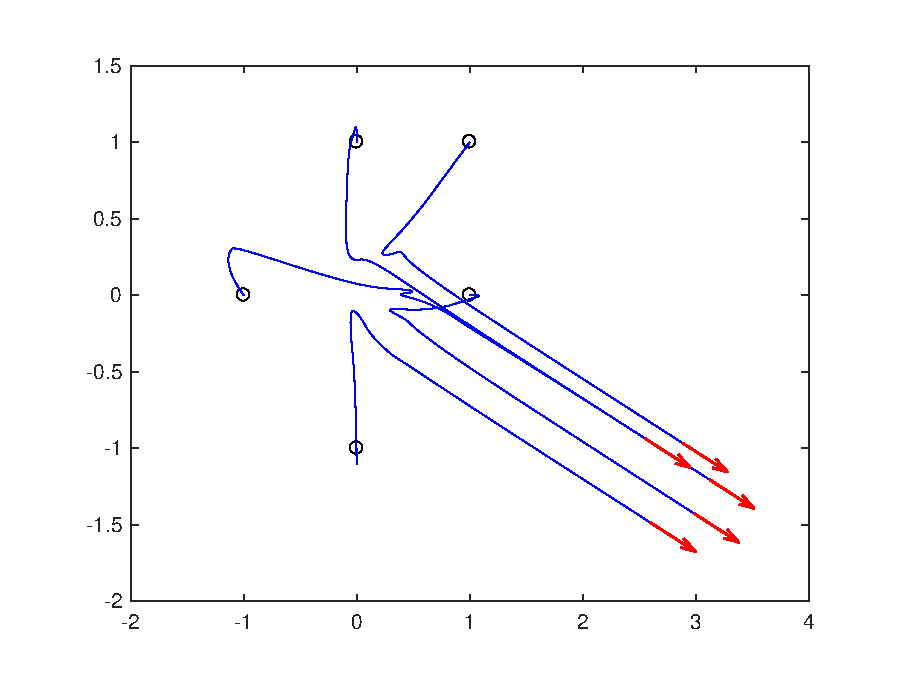
\includegraphics[width=\textwidth]{figures/a5D_L+V_fine_mesh_NICE_ev.eps}
    \caption{Evolution of the system}
    \label{ev}
  \end{minipage}
  \hfill
  \begin{minipage}[b]{0.5\textwidth}
    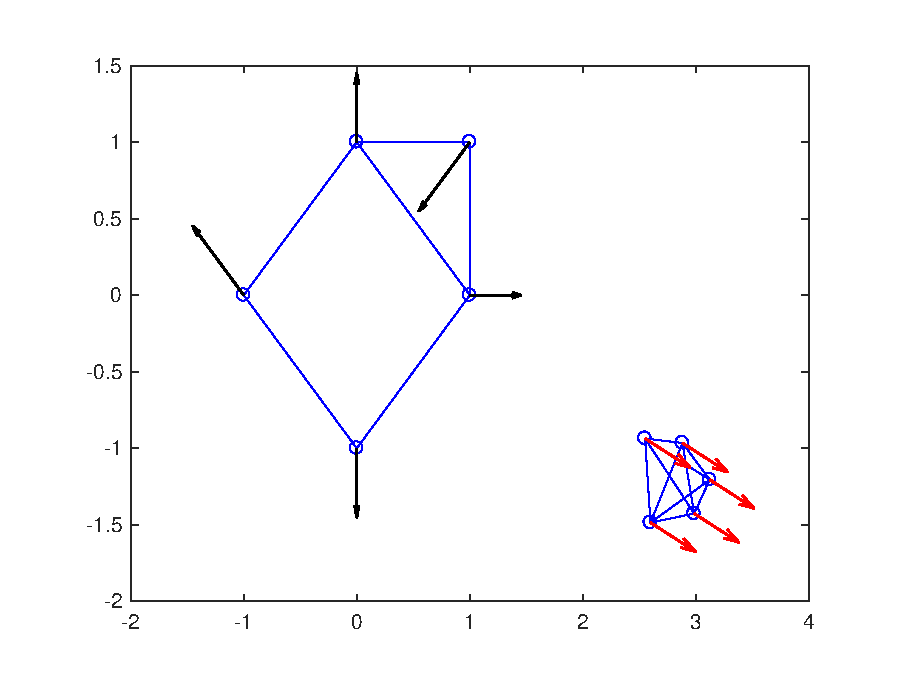
\includegraphics[width=\textwidth]{figures/a5D_L+V_fine_mesh_NICE_g.eps}
    \caption{Initial and terminal configurations}
    \label{g}
  \end{minipage}
\end{figure}

\begin{figure}[ht]
  \begin{minipage}[b]{0.5\textwidth}
    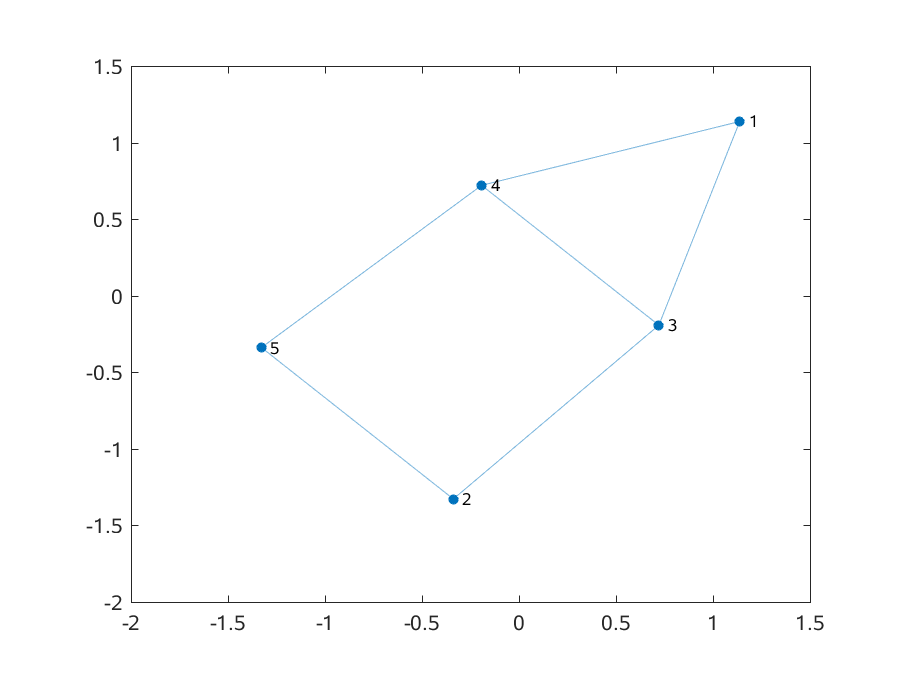
\includegraphics[width=\textwidth]{figures/a5D_L+V_fine_mesh_NICE_cg0.eps}
    \caption{Connectivity at the initial configuration}
    \label{g0}
  \end{minipage}
  \hfill
  \begin{minipage}[b]{0.5\textwidth}
    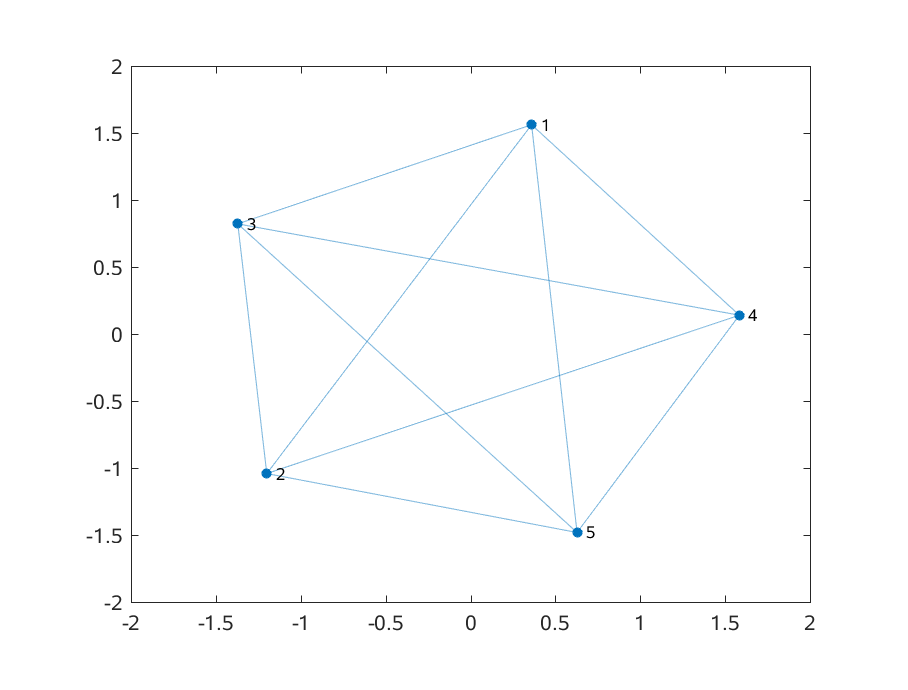
\includegraphics[width=\textwidth]{figures/a5D_L+V_fine_mesh_NICE_cgT.eps}
    \caption{Connectivity at the terminal configuration}
    \label{gT}
  \end{minipage}
\end{figure}
  
 
 \begin{figure}[ht]
 \centering
 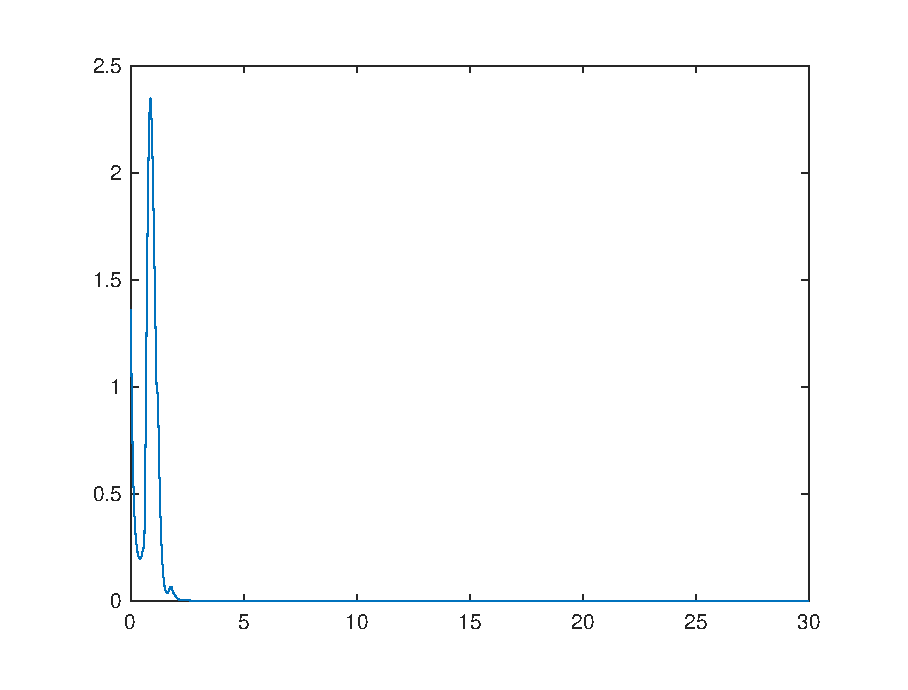
\includegraphics[scale=0.5]{figures/a5D_L+V_fine_mesh_NICE_lv.eps}
 \caption{Lyapunov function}
 \label{lf}
 \end{figure}
  \newpage
The evolution of the system can be observed on the Figure \ref{ev1}. On the Figure \ref{lf} we see the velocity deviation throughout the evolution. The bump in the velocity deviation $B(v(t), v(t))$
is due to the fact that initially the control steers the agents towards each other and after the completeness of the network graph (see Figure \ref{gT}) is reached it brings smoothly the system to consensus with terminal value of velocity deviation $B(v^{mn}, v^{mn}) = 4.21e-07$. Under such terminal configuration the system has entered the consensus region since quantity $E(x^{mn}, v^{mn}) = -0.50$ has become negative and the system tends to consensus uncontrolled.
 
%a10D_L+V_fine_mesh_NICE_lv.eps
We also  consider a \textquotedblleft worse-case\textquotedblright setting involving 10 agents with initial configuration (Figure \ref{g1}) situated on a  zig-zag line forming a minimally connected network at the initial time. The evolution of the system has been illustrated in Figure \ref{ev1} for $T = 30$ and radius of interaction $R = 2$, the number of MPC time windows was chosen $m = 80$  and discretization grid with $n = 40$ grid-points.  On Figure \ref{lf} is plotted the velocity deviation of the group $B(v(t), v(t))$. We observe how the system struggles to maintain the connectivity of the network throughout the evolution, in the end, after the completeness of the network graph is restored (Figure \ref{gT1}), it tends to consensus with terminal value of velocity deviation $B(v^{mn}, v^{mn}) = 1.83e-07$. Here again the consensus region is reached since $E(x^{mn}, v^{mn}) = -0.35$ is negative. 
 


\begin{figure}[ht]
  \begin{minipage}[b]{0.5\textwidth}
    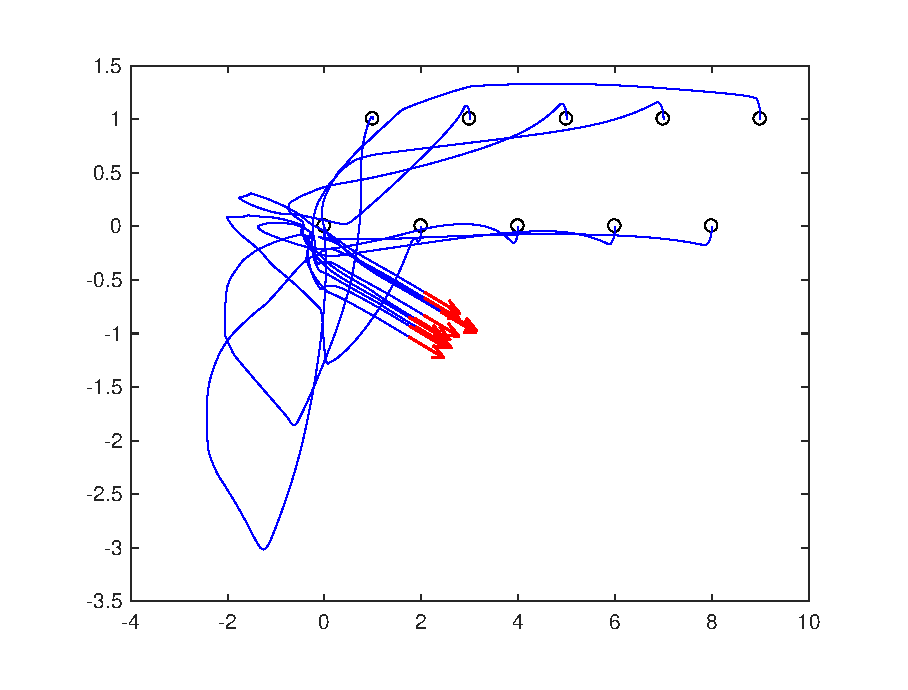
\includegraphics[width=\textwidth]{figures/a10D_L+V_fine_mesh_NICE_ev.eps}
    \caption{Evolution of the system}
    \label{ev1}
  \end{minipage}
  \hfill
  \begin{minipage}[b]{0.5\textwidth}
    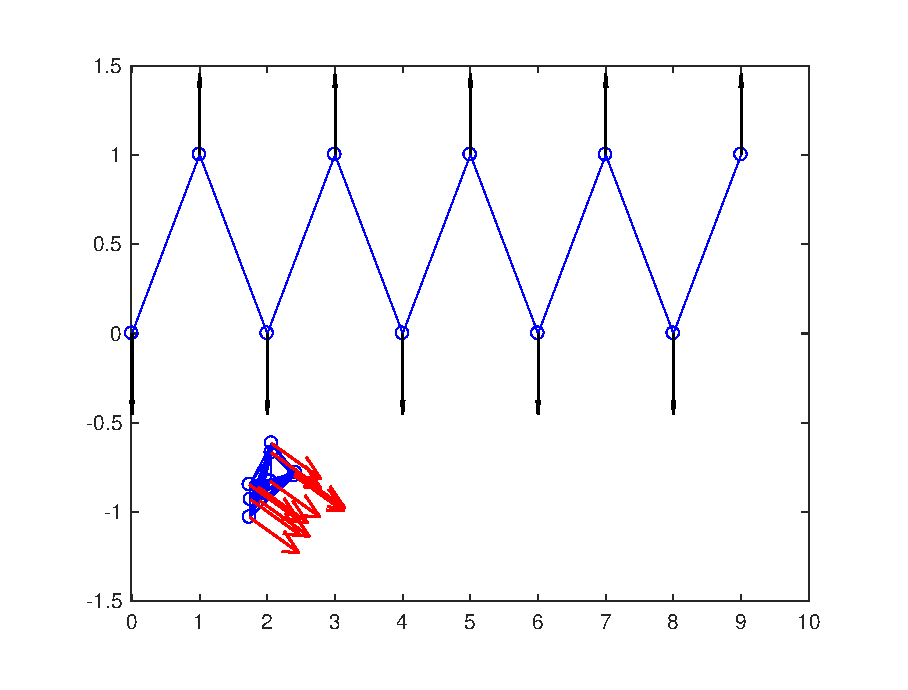
\includegraphics[width=\textwidth]{figures/a10D_L+V_fine_mesh_NICE_g.eps}
    \caption{Initial and terminal configurations}
    \label{g1}
  \end{minipage}
\end{figure}


\begin{figure}[ht]
  \begin{minipage}[b]{0.5\textwidth}
    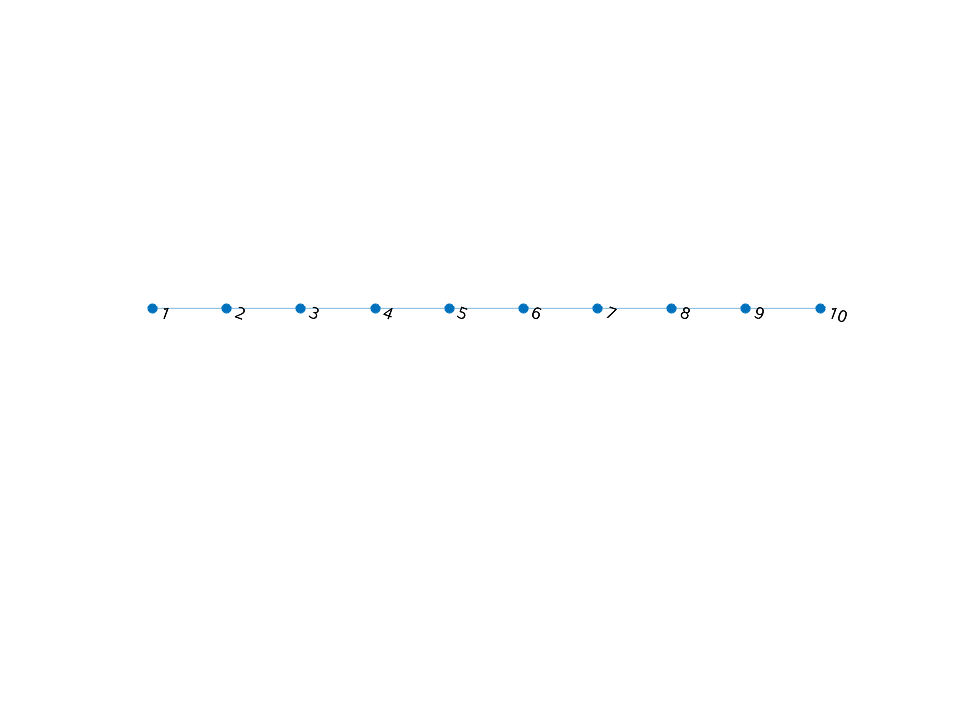
\includegraphics[width=\textwidth]{figures/a10D_L+V_fine_mesh_NICE_cg0.eps}
    \caption{Connectivity at the initial configuration}
    \label{g01}
  \end{minipage}
  \hfill
  \begin{minipage}[b]{0.5\textwidth}
    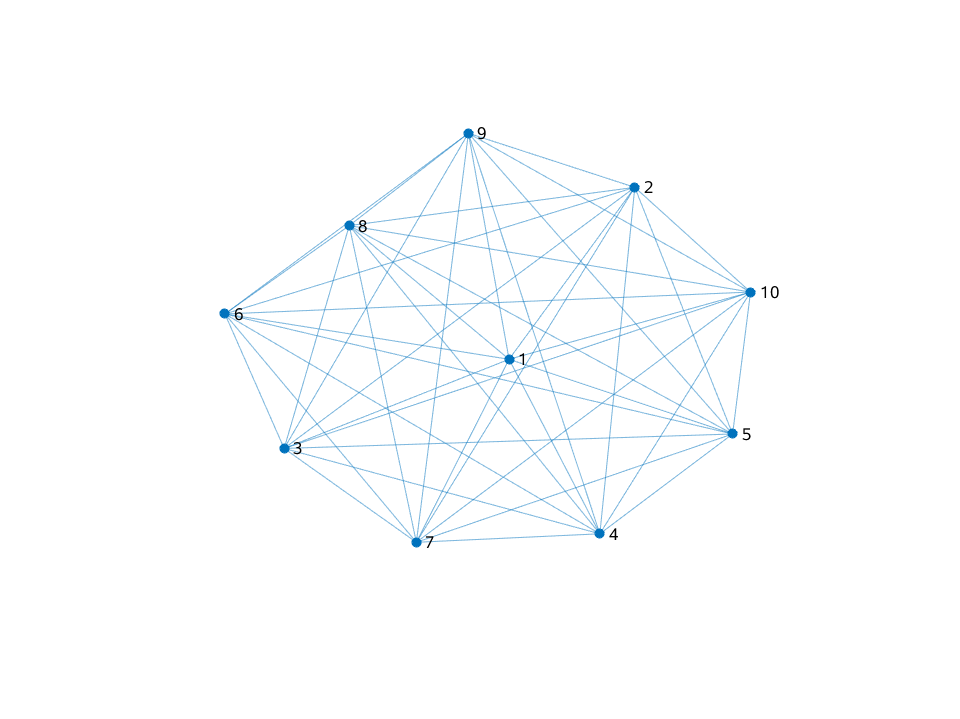
\includegraphics[width=\textwidth]{figures/a10D_L+V_fine_mesh_NICE_cgT.eps}
    \caption{Connectivity at the terminal configuration}
    \label{gT1}
  \end{minipage}
\end{figure}
  
 
 \begin{figure}[ht]
 \centering
 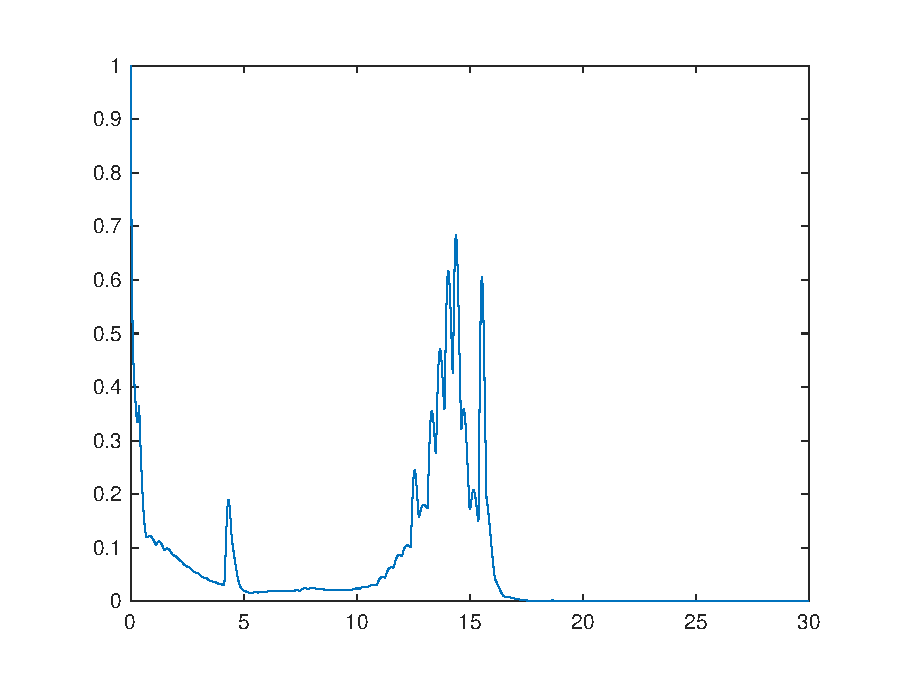
\includegraphics[scale=0.5]{figures/a10D_L+V_fine_mesh_NICE_lv.eps}
 \caption{Lyapunov function}
 \label{lf1}
 \end{figure}
  \newpage









\end{document}
